
%Juan Pablo Roodríguez (jp.rodriguezb1@uniandes.edu.co)

\documentclass[pdftex,12pt,xcolor=pdftex,table]{beamer}
\usepackage{comment}
\usepackage{etex}
\usepackage{amsmath}
\usepackage{amsthm}
\usepackage{amsfonts}
\usepackage{amssymb}
\usepackage{latexsym}
\usepackage{mathtools}
\usepackage{hyperref}
\usepackage{xcolor}
\usepackage[english]{babel}
\usepackage[utf8]{inputenc}
\usepackage{tikz}
\usetikzlibrary{calc,matrix,shapes,arrows}
\usepgflibrary{shapes.arrows}
\usetheme[progressbar=frametitle]{Boadilla}
\setbeamertemplate{frame numbering}[fraction]
\usecolortheme{spruce}
\setbeamercolor{background canvas}{bg=white}

\definecolor{mygreen}{rgb}{.125,.5,.25}
\usecolortheme[named=mygreen]{structure}

\title[Religion in Growth and Happiness]{Does Religion Affect Economic Growth And
Happiness? Evidence From Ramadan} % The short title appears at the bottom of every slide, the full title is only on the title page

\author{Andrés Ramírez \& Juan Pablo Rodríguez} 
% Your name
\institute[]{Summer School of Economics}
\date{June 18, 2020} % Date, can be changed to a custom date

\begin{document}

\begin{frame}
\titlepage
\end{frame}

\begin{frame}{Abstract}
\begin{footnotesize}

\textit{"We study the economic effects of religious practices in the context of the
observance of Ramadan fasting, one of the central tenets of Islam. To establish
causality, we exploit variation in the length of daily fasting due to the interaction
between the rotating Islamic calendar and a country’s latitude. We report
two key, quantitatively meaningful results: (i) longer Ramadan fasting has a
negative effect on output growth in Muslim countries, and (ii) it increases subjective
well-being among Muslims. We find evidence that these patterns are
consistent with a standard club good explanation for the emergence of costly
religious practices: increased strictness of fasting screens out the less committed
members, while the more committed respond with an increase in their
relative levels of participation. Together, our results underscore that religious
practices can affect individual behavior and beliefs in ways that have negative
implications for economic performance, but that nevertheless increase subjective
well-being among followers."}
\\\

Authors: Filipe Campante \& David Yangizawa-Drott (2015)
\end{footnotesize}
\end{frame}

\begin{frame}
\frametitle{Overview}
\tableofcontents 
\end{frame}

\section{Introduction}
    \begin{frame}{Introduction}
        \begin{itemize}
     \item<1-> \vspace {One fundamental aspect that is common to all forms of religion is that they prescribe rules of behavior, or practices, that constrain followers, with varying degrees of strictness.}
     
     \item<2-> \vspace {The recent empirical literature that has studied the relationship between religion and economic performance has found a negative correlation between religious behavior and economic growth, and between religiosity and income at the cross- country and individual levels.}
        \end{itemize}
         
    \end{frame}
    

    \begin{frame}{Introduction}
        \begin{itemize}
     \item<1-> \vspace {The intention is to estimate causal effect of the strictness of a religious practice on economic growth, focusing on the specific example of fasting in observance of the Islamic holy month of Ramadan.}
     
     \item<2-> \vspace {The case of Ramadan illustrates that religious practices can entail significant implications at the aggregate level, while still providing measurable benefits, at least partly due to their role as costly screening devices}
     
     \item<3-> \vspace {focus on costly religious practices, and other aspects of religion could have much different effects.}
     
        \end{itemize}
    \end{frame}    
    
\begin{frame}{Introduction}{Related Literature}
    \begin{itemize}
    \item \vspace {Support of the club good theory of costly religious practices, showing that exogenous variation in strictness leads to screening, and changes in religious engagement, as predicted by the economic approach put forth and surveyed by Iannaccone (1992, 1998).}
    \item<2-> \vspace {Relates to a relatively small literature in economics that has studied the effects of Ramadan fasting.}
    \item<3-> \vspace {The text is in line with a recent and growing literature that looks at specific topics such as work ethic (Spenkuch 2011), entrepreneurship (Audretsch, Boente, and Tamvada 2007), loan repayment decisions (Baele, Farooq, and Ongena 2011), and human capital accumulation (Becker and Woessmann 2009), among others.}
    \end{itemize}
\end{frame}
    
\section{Background}
    \begin{frame}[t]{Background}
    \textbf{What is Ramadan?}
    \vspace{0.5cm}
    
    \begin{columns}[onlytextwidth]
    \column{0.5\textwidth}
    Ramadan is the ninth month of the Islamic calendar, and it is considered sacred as the month in which the Prophet Muhammad first received the revelations. It is mostly known because Muslims abstain from food, drink, smoking and sexual relations between dawn and sunset for the whole month. The daily routine includes \textit{suhur} and \textit{iftar} meals, which are a "unique opportunity for socializing".
    \column{0.5\textwidth}
    \begin{figure}[t]
    \, 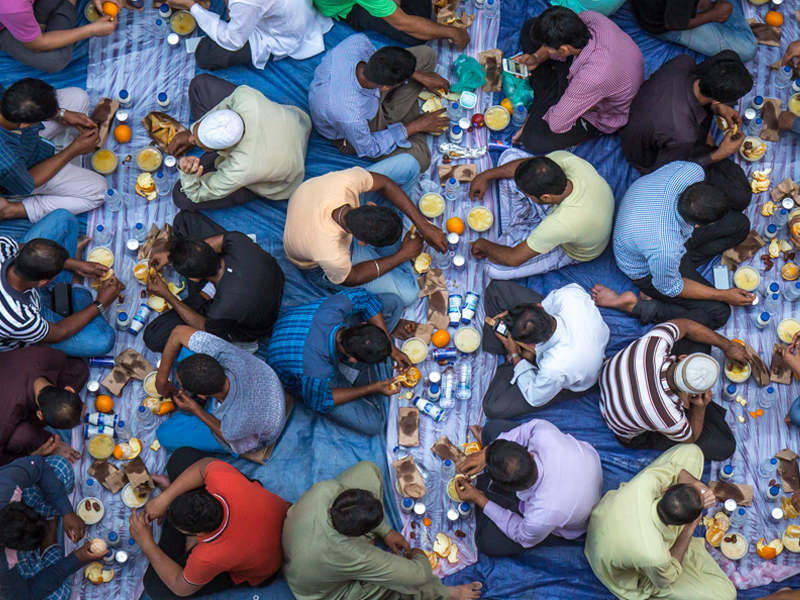
\includegraphics[width=4.5cm, height=5.9cm]{Ramadan-iftar-800px}
    \end{figure}
    \end{columns}
    \end{frame}
    
    \begin{frame}{Background}
    \onslide<1->{Negative consequences}
    \begin{itemize}
    \item \onslide<2->{Physiological: Body weight loss, metabolic changes,irritability, headaches and sleep deprivation (Ziaee et. al, 2006)(Lepiper, Molla \& Molla, 2003)}
    \item \onslide<3->{Prodcutivity: Tiredness, unwillingness to work, reduced level of activity and concentration ability (Afifi,1997)}
    \item \onslide<3->{Lifestyle: There is a considerable reduction in social interactions}
    \end{itemize}
    \onslide<4->{Positive consequences}
    \begin{itemize}
    \item \onslide<5->{Psychological: Tendency to participate in stress reduction and spiritual activities (Afifi,1997)}
    \end{itemize}
    \end{frame}

\section{Empirical Framework}
\subsection{Data}
    \begin{frame}{Empirical Framework}{Data}
    \begin{itemize}
    \item<1-> \vspace {They collect data from the Astronomical Applications Department of the U.S. Naval Observatory to calculate the number of stipulated fasting hours during Ramadan.}
    \item<2-> \vspace {To map historical Ramadan dates from the Islamic calendar to the Gregorian calendar, They use data from Islamic Philosophy Online.}
    \item<3-> \vspace {Match the data on Ramadan fasting hours with various data sets like: data from Version 1.1 of the World Religion Project, Penn World Tables 8.0 (PWT8.0), national-accounts data on real GDP growth per worker in constant 2005 prices.}
    \item<4-> \vspace {To asses whether Ramadan affects SWB, the authors use data from all six waves of the World Values Survey (WVS).}
    \end{itemize}
    \end{frame}
    
\subsection{Identification Strategy and Specifications}
    \begin{frame}{Empirical Framework}{Identification Strategy and Specification}
    \centering
    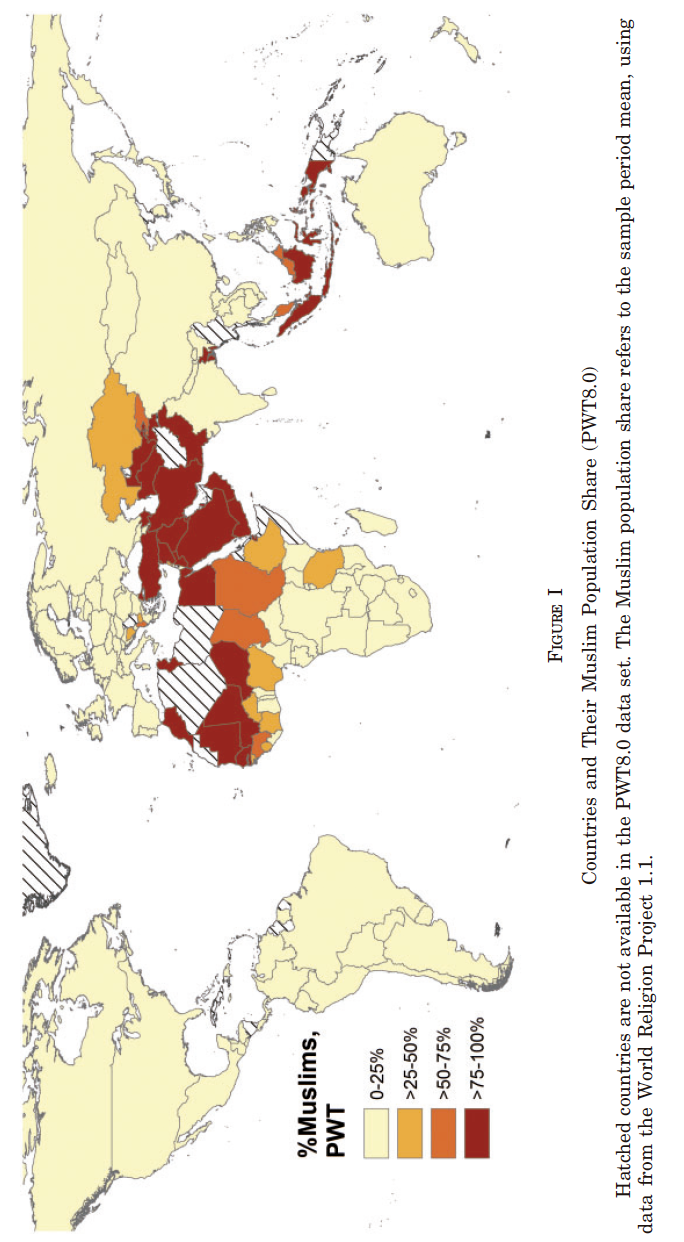
\includegraphics[scale=0.55, angle =270 ]{Map.png}
    \end{frame}
    
    \begin{frame}{Empirical Framework}{Identification Strategy and Specification}
    \begin{itemize}
    \item<1-> In years where Ramadan is held in summer, fasting stands longer. When it is held in winter, fasting is substantially shorter.
    \item<2-> Location plays a huge role in fasting hours. The closer a country is to the equator, the less variant the fasting hours.
    \item<3-> Given that most of the Muslim countries are located in the northern hemisphere, fasting hours fluctuate with the northern seasons.
    \end{itemize}
    \end{frame}
    
    \begin{frame}{Empirical Framework}{Identification Strategy and Specification}
    \centering
    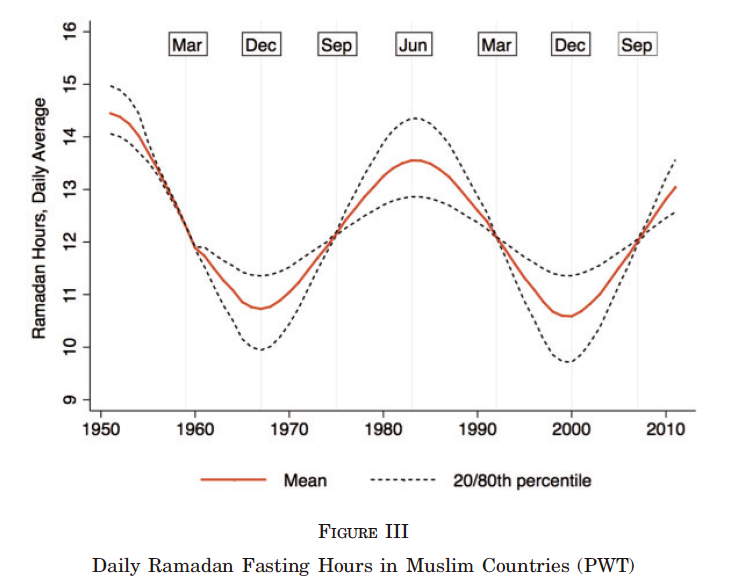
\includegraphics[scale=0.65]{dailyramadan.png}
    \end{frame}
    
    \begin{frame}{Empirical Framework}{Identification Strategy and Specification}
    \begin{equation}
    \nonumber g_{ct}=\beta *RamadanHours_{ct}+\delta_c+\mu_t+\epsilon_{ct}
    \end{equation}
    \vspace{0.5cm}
    \begin{itemize}
    \item<2-> $g_{ct}=$ Real GDP per Worker in country $c$ in year $t$
    \item<3-> $RamadanHours_{ct}=$ Logged average daily number of fasting hours during Ramadan
    \item<4-> $\delta$ and $\mu=$ Country and year fixed effects respectively
    \end{itemize}
    \end{frame}
    
    \begin{frame}{Empirical Framework}{Identification Strategy and Specification}
    \begin{equation}
    \nonumber g_{ct}=\beta(RamadanHours_{ct})*(Muslim_{ct})+\lambda(RamadanHours_{ct})
    
    +X_{ct}\gamma+\delta_c+\mu_t+\epsilon_{ct}
    \end{equation}
    \vspace{0.5cm}
    \begin{itemize}
    \item<2-> $Muslim=$ Share of Muslims in the population
    \item<3-> $X=$ Vector of covariates consisting of flexible controls of the Muslim population share
    \end{itemize}
    \end{frame}
    
    \begin{frame}{Empirical Framework}{Identification Strategy and Specification}
    \begin{equation}
    \nonumber y_{ict}=\beta*RamadanHours_{ct}*+X_{ict}\gamma+\delta_c+\mu_t+\epsilon_{ict}
    \end{equation}
    \vspace{0.5cm}
    \begin{itemize}
    \item<2-> $y=$ subjective well-being for individual $i$, of country $c$ and 
    
    year $t$
    \item<3-> $X=$ Vector of demographic control
    \end{itemize}
    \end{frame}
    
\section{Basic Results}

\subsection{Effects on Economic Growth}

    \begin{frame}{Basic Results}{Effects on Economic Growth}
    \vspace{-0.57cm}
    \centering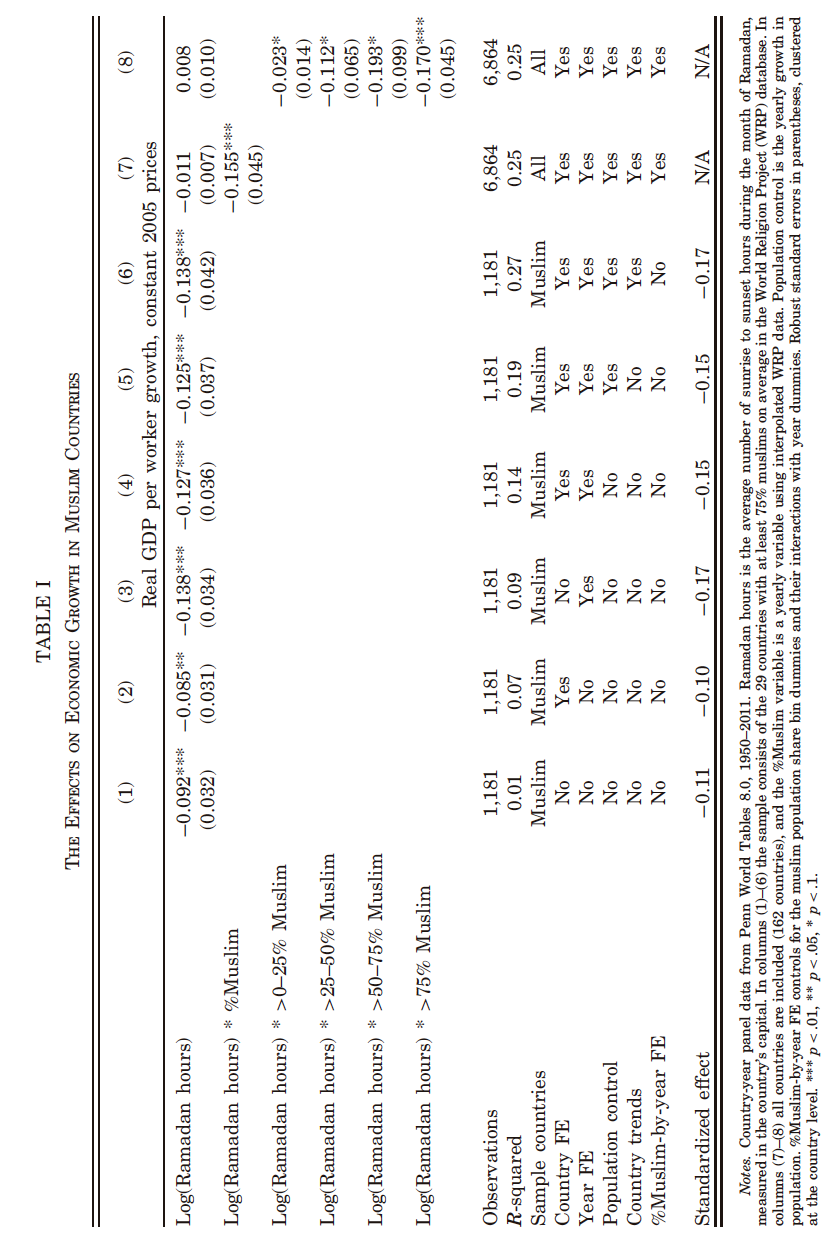
\includegraphics[scale=0.5, angle =270 ]{reg1.png}
    \end{frame}
    
    \begin{frame}{Basic Results}{Effects on Economic Growth}
    \begin{itemize}
        \item Results from columns (1) to (6) show the following (specification 1):
        \begin{itemize}
            \item<2-> Not including country FE and/or not controlling for population growth generate an overestimation of the coefficient that explains the effect of $RamadanHours_{ct}=$ in the GDP per worker of Muslim countries
            \item<3-> The opposite effect is happens when not including year FE or not controlling for country linear trends
            \item<4-> We show that the quantity of fasting hours have a negative effect on the GDP per worker in every case
        \end{itemize}
    \end{itemize}
    \end{frame}
    
    \begin{frame}{Basic Results}{Effects on Economic Growth}
    \begin{itemize}
        \item Results from column (7) show the following (specification 2):
        \begin{itemize}
            \item<2-> Non-Muslim countries are not affected substantially by their amount of fasting hours
            \item<3-> As we saw in (1) to (6), Muslim countries are significantly affected in their economic growth by the amount of fasting hours
        \end{itemize}
        \item<4-> Results from column (8) show the following (altered specification 2):
        \begin{itemize}
            \item<5-> This regression is a lot more precise in terms of the share that Muslims should represent in the population for Ramadan´s fasting hours to have an effect. We can see that, with a 5\% as a level of significance, only countries with a 75\% or higher are truly affected.
        \end{itemize}
    \end{itemize}
    \end{frame}
    
    \begin{frame}{Basic Results}{Effects on Economic Growth}
    \centering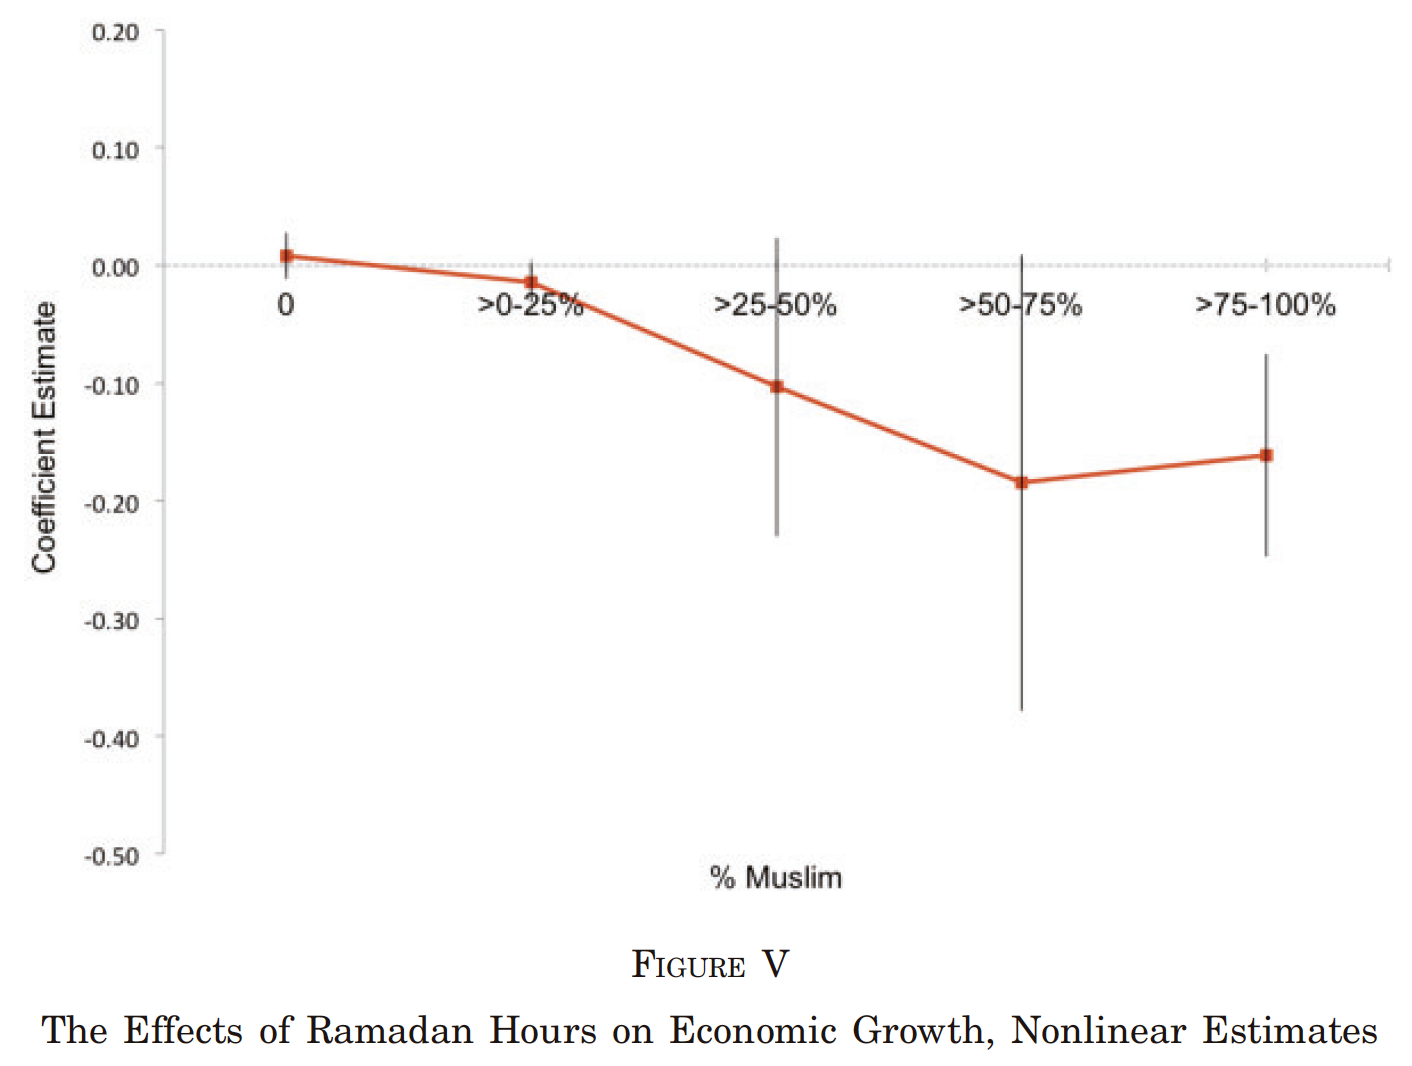
\includegraphics[scale=0.37]{POIC.png}
    \end{frame}
    
\subsection{Effects on Subjective Well-Being}
    \begin{frame}{Basic Results}{Effects on Subjective Well-Being}
    \vspace{-0.57cm}
    \centering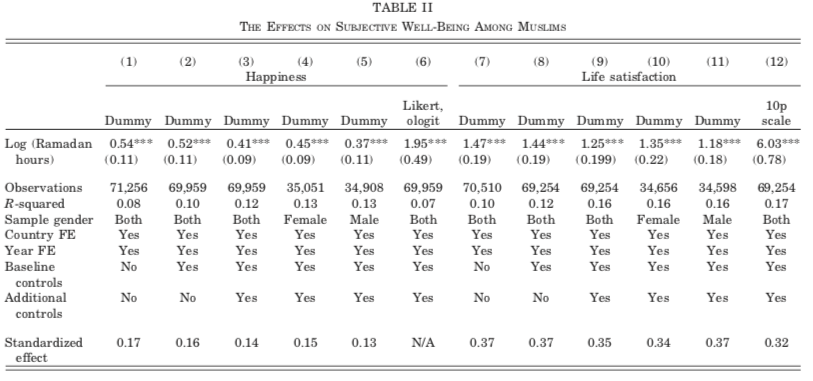
\includegraphics[scale=0.4]{Reg2.png}
    \end{frame}
    
   \begin{frame}{Basic Results}{Effects on Subjective Well-Being}
     \begin{itemize}
        \item From columns (1) and (2) is possible to analize that Ramadan fasting increases measured SWB for Muslim individuals:
        \begin{itemize}
            \item<2-> Coefficients are positive and statistically significant (p $< .001$).
            
        \end{itemize}
        \item<3-> Columns (3) and (4) estimate the effects separately for men and women:
        \begin{itemize}
            \item<4-> The coefficients are significant and positive for both sexes, with a point estimate of slightly larger magnitude for women.
        \end{itemize}
        \item<5-> The results are robust to two-way clustering of the standard errors and controls for country-specific trends.
        \item<6-> In summer Ramadans, Muslims would be about 5 percentage points likelier to report they are happy.
    \end{itemize}
    \end{frame}    
 
\section{Discussion}
\subsection{Costly Religious Practices}
    \begin{frame}{Discussion}{Costly Religious Practices}
    What explains the effect of religion on subjective  well-being? 
    \begin{itemize}
        \item<2-> A key idea in literature is that the utility obtained by an individual from her religious activities increase in function of the engagement of her fellow worshipers.
        \item<3-> Increasing the strictness and cost of the practices associated with a religious group can improve the welfare of its members in two ways: 
        \begin{itemize}
            \item<4-> May increase the relative cost of engaging in activities outside the group.
            \item<5-> Strict practices work as a screening device to keep out relatively less committed members or potential members.
        \end{itemize}
        \item<6->  Increasing the strictness of fasting requirements is economically costly, as demonstrated by the impact on economic performance, but can nevertheless be associated with increased SWB.
    \end{itemize}

    \end{frame}


    \begin{frame}{Discussion}{Costly Religious Practices: Membership and Engagement}
    \vspace{0.0cm}
    \centering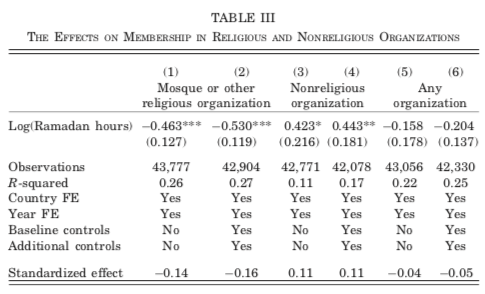
\includegraphics[scale=0.5]{tab3.png}

    \end{frame}


    \begin{frame}{Discussion}{Costly Religious Practices: Membership and Engagement}
    Increasing the strictness of the Ramadan fasting requirement reduces membership of Muslim individuals in religious groups and induces a corresponding increase in mem- bership of other kinds of organizations.
    \begin{itemize}
        \item<2-> Longer Ramadan hours have a negative effect on active member- ship of religious organizations, with and without controlling for individual demographic characteristics.
        \item<3-> this behavior is mirrored by an increase in membership of nonre- ligious organizations, essentially of the same magnitude, such that the likelihood of being an active member of an organization of any kind is unaffected. 
        \item<4-> Increasing the strictness of fasting requirements is economically costly, as demonstrated by the impact on economic performance, but can nevertheless be associated with increased SWB.
      \end{itemize}
    \end{frame}


    \begin{frame}{Discussion}{Costly Religious Practices: Membership and Engagement}
    \vspace{-0.5cm}
    \centering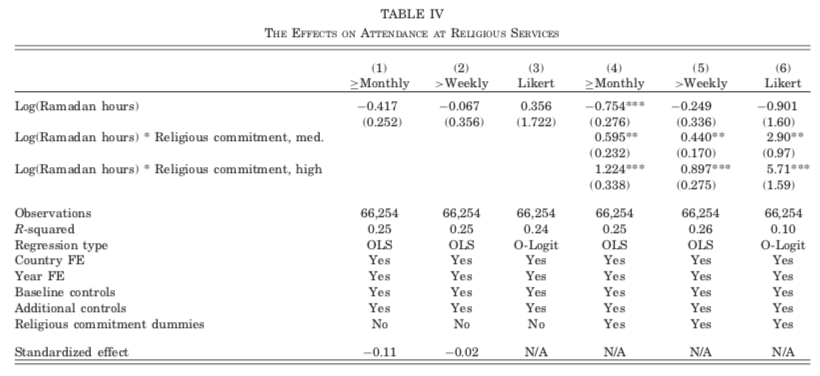
\includegraphics[scale=0.37]{tab4.png}

    \end{frame}
    

    \begin{frame}{Discussion}{Costly Religious Practices: Membership and Engagement}
    The stricter fasting requirement induces less committed individuals to disengage with religious activity: 
    \begin{itemize}
        \item<2-> No significant effect of increased Ramadan fasting on attendance.
        \item<3-> Those who remain committed to the group may actually increase their engagement with in-group activities, as the reduction in free-riding will make participation more appealing 
        \item<4-> The negative main effect of fasting hours, which,  means that those individuals who are predicted to be less committed actually reduce their likelihood of attending a mosque.
        
      \end{itemize}
    \end{frame}
    

    \begin{frame}{Discussion}{Costly Religious Practices: Beliefs}
    \vspace{-0.5cm}
    \centering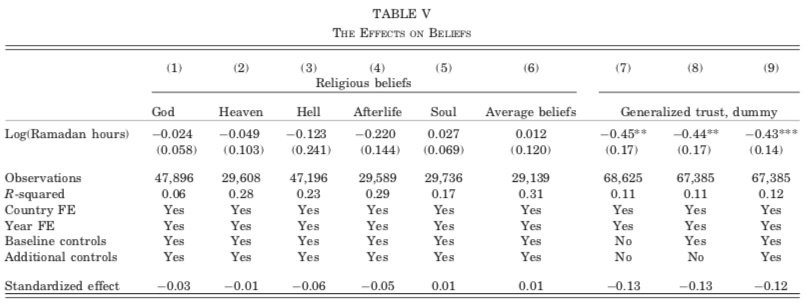
\includegraphics[scale=0.43]{tab5.png}
    \end{frame}  


    \begin{frame}{Discussion}{Costly Religious Practices: Beliefs}
    Increased strictness of fasting requirements has an effect on beliefs and attitudes, not so much in the strictly religious domain, but likely as a result of their impact on patterns of socialization: 
    \begin{itemize}
        \item<2-> No evidence of an effect of increased Ramadan fasting requirements over the prevalence of any of these religious beliefs, nor on the average over the different kinds.
        \item<3-> Longer Ramadan fasting actually has a significant negative effect on generalized trust, with and without the different sets of demographic controls. 
        
      \end{itemize}
    \end{frame}

\subsection{Productivity and Labor Supply}
    \begin{frame}{Discussion}{Productivity and Labor Supply}
    Are effects in economic growth due to an impact on productivity or on input supply decisions?
    \begin{itemize}
        \item<2-> We face a pattern of competing for time and resources between production and religious practices, thereby affecting input supply.
        \item<3-> It is evident the existence of psychological consequences, that, although there is a possibility of mitigation given an increased networking, will produce a negative effect on labor productivity.
        \item<4-> Given the presented data,we can show that Ramadan has longer-lasting effects beyond the given month
    \end{itemize}
    \end{frame}
    
    \begin{frame}{Discussion}{Productivity and Labor Supply}
    \vspace{-0.5cm}
    \centering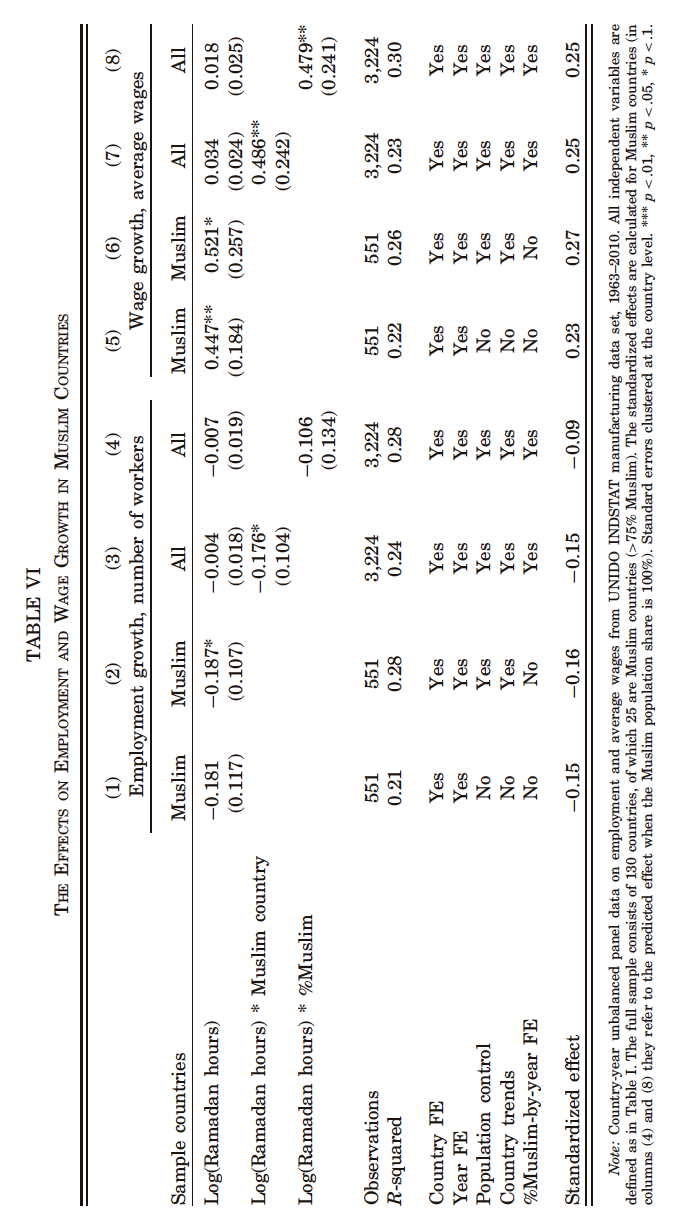
\includegraphics[scale=0.55, angle=270]{Reglabor.png}
    \end{frame}
    
    \begin{frame}{Discussion}{Productivity and Labor Supply}
    \begin{itemize}
        \item \onslide<1->{We can see that the labor market does not behave as basic economic theory dictates, the regression could not prove the impact of Ramadan in employment growth or salary levels.}
        \item \onslide<2->{Still the paper's appendix shows that Ramadan causes a positive effect on people willingness to put religion over work or leisure.}
        \item \onslide<3->{There is a possibility of endogeneity due to a measurement error, given that most of the Muslim countries are emerging economies and a fairly share of its labor market is not formal.}
        
        \vspace{0.5cm}
        \onslide<4->{Note: Productivity reduction proof is given earlier on the presentation.}
    \end{itemize}
    \end{frame}
    

\section{Concluding Remarks}
    \begin{frame}{Concluding Remarks}
    
    \begin{itemize}
        \item<1-> There is causal evidence for a negative effect of the length of Ramadan fasting on the economic growth of Muslim countries.
        \item<2-> There is causal evidence for a positive effect of the length of Ramadan fasting on the self-reported happiness and life satisfaction.
        \item<3-> There is a bunch of channels in which fasting affects economic performance and becomes a costly religious practice within the economy or even the culture itself
        \item<4> This article provides new insights for the ongoing debate regarding how to asses the effects of policy interventions on welfare.
    \end{itemize}
        
    \end{frame}
    
\begin{frame}{References and Contact Information}
    Campante, F. and Yanagizawa-Drott, D., 2015. "Does religion affect economic growth and happiness? Evidence from Ramadan. The Quarterly Journal of Economics, 130(2), pp.615-658.
    \begin{itemize}
        \item \href{http://qje.oxfordjournals.org/content/130/2/615.full.pdf+html}{\textcolor{blue}{\underline{Paper link}}}
        \item \href{https://yanagizawadrott.com/wp-content/uploads/2016/02/rwandadyd_appendix_aug2014.pdf}{\textcolor{blue}{\underline{Appendix}}}
        \item \href{https://sites.google.com/view/prof-filipe-campante/home}{\textcolor{blue}{\underline{Filipe Campante personal website}}}
        \item \href{https://yanagizawadrott.com/}{\textcolor{blue}{\underline{David Yanagizawa-Drott personal website}}}
      \end{itemize}
    Contact Information:
    \begin{itemize}
        \item Andrés Ramírez - andrese.ramirez@urosario.edu.co
        \item Juan Pablo Rodríguez - jp.rodriguezb1@uniandes.edu.co
    \end{itemize}
        
    
\end{frame}

\end{document}